%-----------------------------------------------------------------------------------------------------------------------------------------
% PACKAGES
%Document Class starts every LaTeX document.  In this case, we're declaring the document class to be a book.  Changing "oneside" to "twoside" changes where the page numbers and headers and such get placed.
\documentclass[12pt,oneside]{book}

%These are the packages I used.  There's a description of (most of) them below (that Arthur wrote):
\usepackage{fancyhdr, geometry, graphicx, epstopdf, lscape, setspace, amssymb, amsmath, wasysym,moreverb, natbib, titlesec, longtable, multirow, alltt,here, indentfirst,ifthen}

\usepackage[small,bf]{caption}
\geometry{letterpaper}


%The "raggedbottom" command allows LaTeX to take some liberty with where the text on a page ends. This saved me some weird formatting problems I was having.
 \raggedbottom
 
%set the pagestyle:
\fancypagestyle{plain}{
\fancyhf{} % clear all header and footer fields, we will re-format them later

%Some formatting stuff:
\renewcommand{\headrulewidth}{0pt}
\renewcommand{\footrulewidth}{0pt}}
\newcommand{\nat}{Nature}

%	NECESSARY PACKAGES
%	fancyhdr enables use of fancy pagestyle
%	geometry defines page layout
%	graphicX allows for inclusion of graphics and page scaling and rotation
%	epstopdf allows the conversion of eps files to pdf and is required for figures
%	caption allows the captioning of figures
%	lscape allows for the creation of landscape pages-- important for large tables
%	setspace allows for doublespacing
%	natbib allows for the citations and Bibtex
%	titlesec allows for the definition of title layouts

%	OPTIONAL PACKAGES
%	aastex is only useful for article submission
%	revsymb is for physics symbols
%	amssymb is for math symbols
%	amsmath is for math formatting for things like matrices
%	parskip (\usepackage[parfill]{parskip})  allows paragraphs to begin with empty line
%	mathrsfs is required for \mathscr, the best Lagrangian and FT font
%	here makes !h force graph here and !t force the graph at the top of the page
%	wrapfig allows the wrapping of figures
%	fontspec allows the specification of fonts
%	color allows for the specification of the color of fonts
%	eso-pic allows the addition of watermarks such as a draft date


%-----------------------------------------------------------------------------------------------------------------------------------------
% RULES

%This has something to do with headers and margins and stuff:
\DeclareGraphicsRule{.tif}{png}{.png}{`convert #1 `dirname #1`/`basename #1 .tif`.png}
\textwidth 5.750in \textheight=8.50in \headheight 0.0625in \topmargin 0.0in % book strict

%==============================================================================
% Uncomment below for one sided printing (margins the same on even and odd pages)
\oddsidemargin 0.500in \evensidemargin 0.500in

% Uncomment below for two sided printing (margins different on even and odd pages)
%\oddsidemargin 0.563in \evensidemargin 0.2500in

%This sets how we want the formatting of chapter titles to look (bold face and Huge):
\titleformat{\chapter}{\bf\Huge}
{Chapter \thechapter}{-4.4em}{\\}
\titlespacing*{\chapter}{0pt}{-.57in}{*3}

%This formats the section headings:
\titleformat{\section}{\bf\Large}
{\thesection}{1em}{}
\titlespacing*{\section}{0pt}{*2}{*2}

%Let's double-space the document:
\doublespacing

%And our citation style will be aa (astronomy style):
\citestyle{aa}

%-----------------------------------------------------------------------------------------------------------------------------------------
% DOCUMENT/ TITLE PAGE
%Now the document actually begins:
\begin{document}

%This states that this is the stuff that comes before the real text:
\frontmatter

%Here goes the title page:
\pagestyle{empty}
\begin{titlepage}
\begin{center}
\rule{5.75in}{1pt} \\
\vspace*{-0.125in}
{\large \doublespacing Wesleyan University} \hfill {\large \doublespacing The Honors College}
\rule[0.2in]{5.75in}{1pt} \\
\vspace*{0.8in}
{\LARGE \singlespacing \bf Necroplanetology: \\ Dead Planets \\Are Fun} \\
\vspace*{0.05in}
\vspace*{0.10in}
{\large \vspace*{0.20in}  \singlespacing by \vspace*{.2in}
\\Girish Duvvuri \\ Class of 2017\\}
\vspace*{0.25in}
\vspace*{0.8in}
{\large \singlespacing A thesis submitted to the\\ faculty of Wesleyan University\\ in partial fulfillment of the requirements for the \\ Degree of Bachelor of Arts\\ with Departmental Honors in Astronomy\\ \vspace*{-0.15in} }
\vspace*{.25in}
\rule{5.75in}{1pt} \\
\vspace*{-0.125in}
{\large \doublespacing Middletown, Connecticut \hfill Eventually, 2048}
\rule[0.2in]{5.75in}{1pt} \\
\end{center}
\end{titlepage}


%-----------------------------------------------------------------------------------------------------------------------------------------
% ABSTRACT/ ACKNOWLEDGEMENTS
%After the title page, comes anything else you want before the Table of Contents.  Note that the Epigraph and acknowledgements are in their own files.  The \include command inserts the external files into the final document.

\pagestyle{empty}
%\pagestyle{plain}

\mbox{}
\vspace{.75in}
\hrule

\vspace{2in}


%\begin{minipage}[c]{4in}
\begin{centering}
	\hspace{.25in} 
	\parbox{5in}{
		\noindent 
		\textit{Well Shit.}
		\vspace{3pt}

		\begin{flushright}
			{\sc {--Varric Tethras}}\\
			{\textit{Dragon Age Inquisition}}
		\end{flushright}
	}
\end{centering}
\vspace{2.25in}
\hrule
\vfill



%\flushleft















\textwidth 5.750in \textheight=8.50in \headheight 0.0625in \topmargin 0.0in % book strict



\chapter*{Acknowledgements}



\titlespacing*{\chapter}{0pt}{*2}{*3}
Thank you D.S. (for sending) and H.R.S. (for making).

%My title formatting changes after the frontmatter, because of how i formatted my acknowledgements:

\titleformat{\chapter}{\bf\Huge}
{Chapter \thechapter}{-4.4em}{\\}
\titlespacing*{\chapter}{0pt}{*2}{*3}

\titleformat{\section}{\bf\Large}
{\thesection}{1em}{}
\titlespacing*{\section}{0pt}{*2}{*2}


%-----------------------------------------------------------------------------------------------------------------------------------------
% CONTENTS/ RULES OF HEADERS
%LaTeX creates a table of contents for you automatically, but you may have to compile the document twice before it shows up properly:

\tableofcontents  \pagestyle{empty}

%You can also put in the following, if you wish:

%\listoffigures
%\listoftables \pagestyle{empty}


%Now we start the real part of the document:
\mainmatter


%-----------------------------------------------------------------------------------------------------------------------------------------
% HEADERS
%This took me forever to figure out properly, and you may want to change it.  There's also different thing you can do if you want doublesided printing.  Your final thesis, as published by the University, is one-sided.


\renewcommand{\chaptermark}[1]{ \markboth{\sc\thechapter.\ #1}{}}

\pagestyle{fancy}
\fancyhead{}
\fancyfoot{}

\fancyhead[L]{\leftmark}
\fancyhead[R]{\thepage}

%==============================================================================
%Number your pages!  
\pagenumbering{arabic}

%-----------------------------------------------------------------------------------------------------------------------------------------
% CHAPTERS
%Here's the actual thesis:  (note that file names CAN'T have spaces in them!)

\chapter{Introduction}
\label{intro}

Background Info on white dwarfs and exoplanetary systems:
\section{Exoplanets}
Rise of the field, importance for understanding diversity of planetary systems
Context for pulsar planet as first exoplanet detection, lead in to post-stellar evolution objects. 

\textbf{Work notes:} mostly text, lit review.
\section{Transits}
Introduction to transit method (not very long)
Discussion of why WDs are favorable for transit detections: comparison figure of lightcurves for Earth transiting Sun vs WD

\textbf{Work notes:} mostly text, lit review. Make one figure.
\section{WD Transit Motivation}
Debris disks+ Polluted WDs: frequency, sinking timescales, overview of past work as motivation for transit studies. We know there are planetary remnants there.
K2 mission and guest proposals.

\textbf{Work notes:} Text. lit review +  go over other K2 guest proposals.
\section{WD1145 Detection}
Details regarding detection and a little information about followup photometry (more in Chapter \ref{chapter_photo}). 
Then \cite{Xu2016} detection of circumstellar absorption, leads into discussion of next section.

\textbf{Work notes:} Do some work with available K2 photometry papers to find the best way to summarize object's behavior. Pick out a stellar line to show CS absorption clearly: strong, isolated, preferably from Xu data to show blue and red edges. Or a more large-scale view like \cite{Xu2016} Fig 1a/b?
\section{Significance of WD1145} 
Explanation of lack of knowledge of planetary interiors: RV + transit constrain Mass/Radius $\implies \rho$, transit and eclispse spectroscopy give atmospheric info, but now we use WD as our mass spectrometer to get information about planetary interior. To give context, list some other known disintegrating planetary systems or other ways we've constrained composition (find the iron exo-Mercury that was identified because its orbital period requires that composition to avoid the disintegration we see here)

\textbf{Work notes:} lots of lit review (bring in work with disks, but not too much because that will get discussed more in Chapter \ref{chapter_spectra})


\section{Figure+Citation}

Look figure + citation: \citep[e.g.,][see Fig. \ref{PrettyPic}]{Vanderburg2015}. 

\begin{figure}
\centering
\scalebox{0.45}{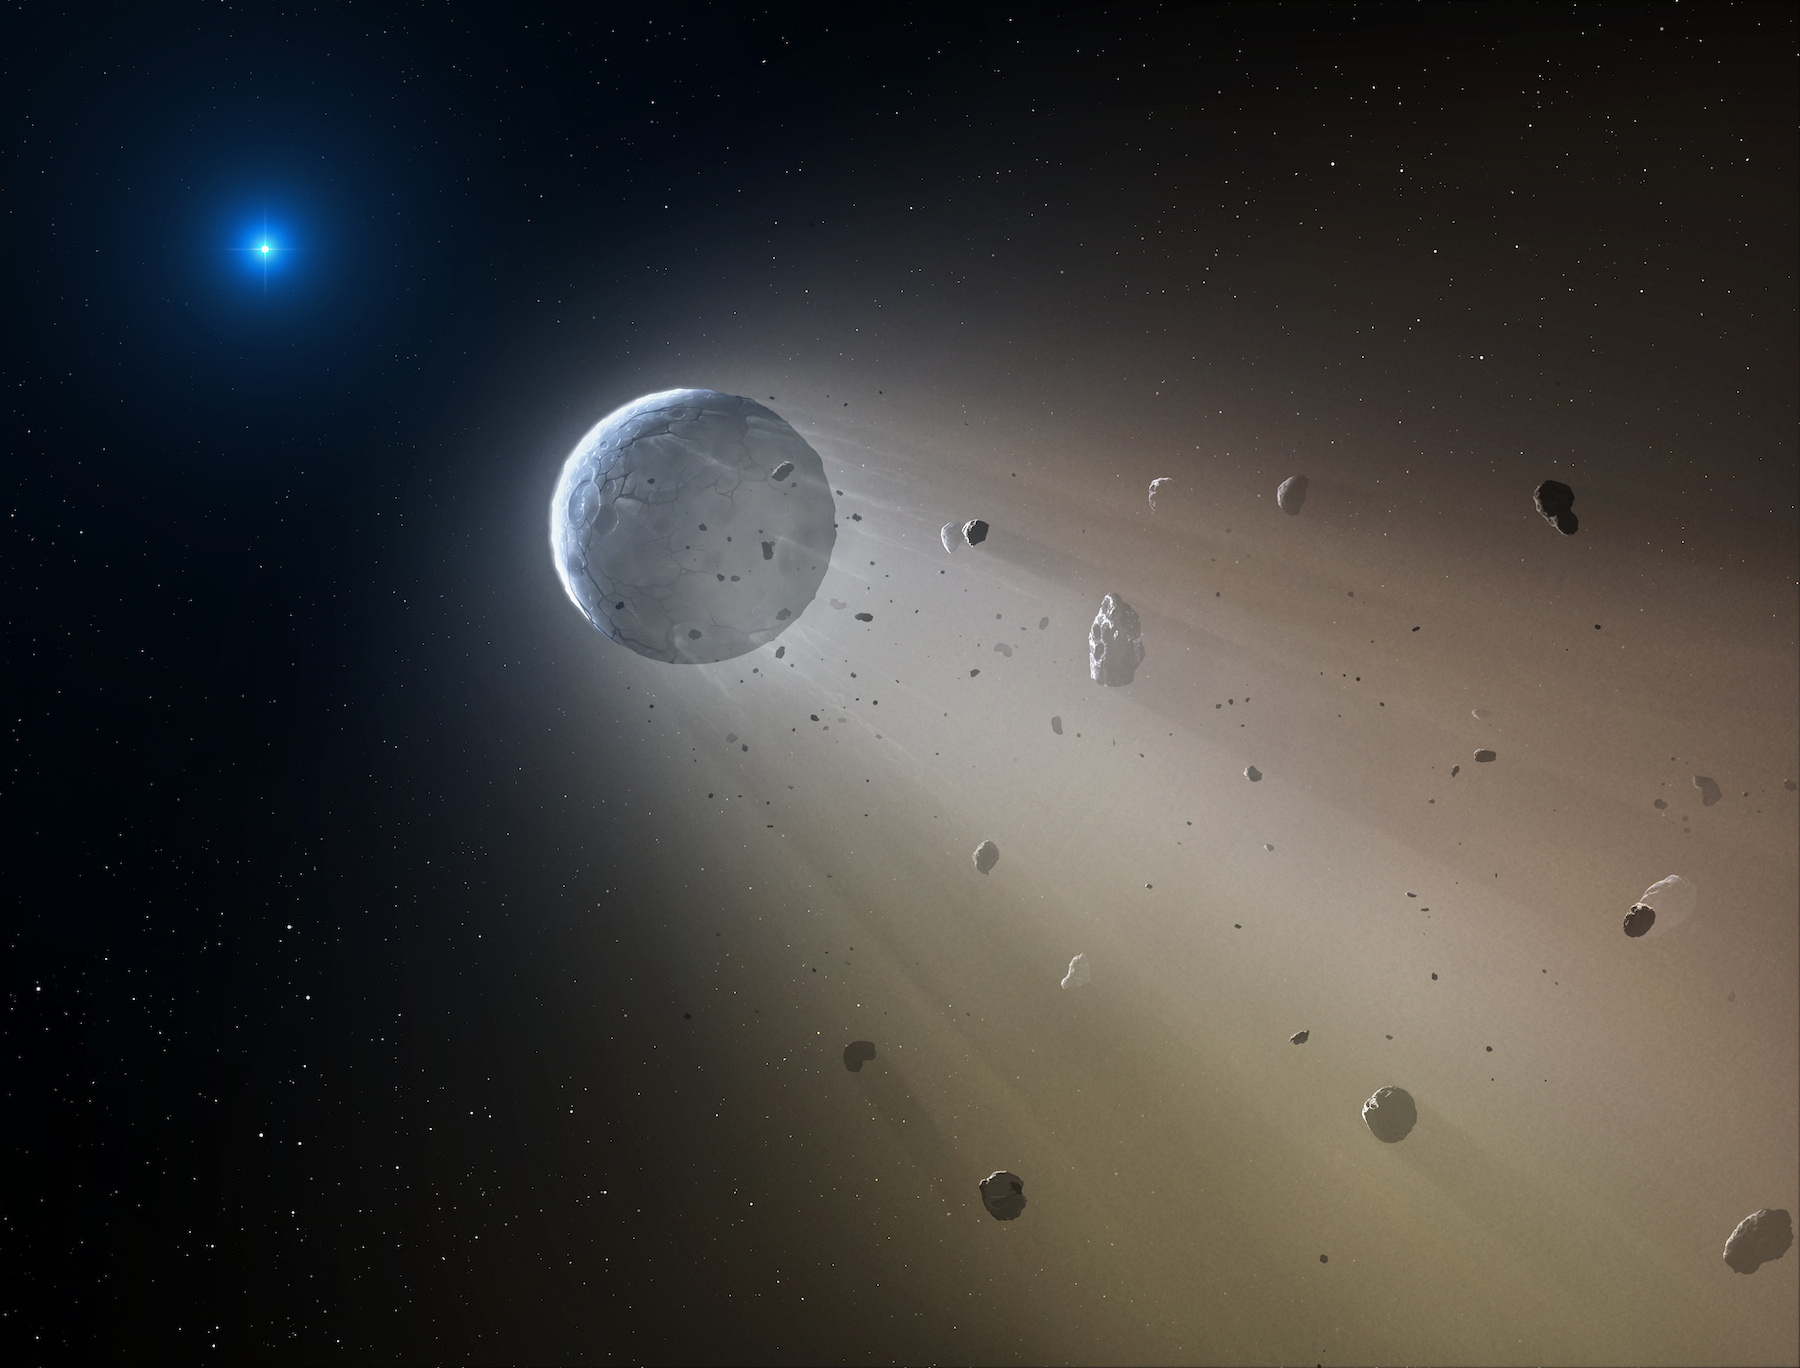
\includegraphics{Figures/PrettyPic.png}}
\caption{The artist rendition of WD1145+017 \citep[from][]{Vanderburg2015}.}
\label{PrettyPic}
\end{figure}

%\ifthenelse{\isodd{\thepage}}{\clearemptydoublepage}{}
\chapter{Spectroscopy}
\label{chapter_spectra}


More info about previous work done with polluted WDs, but then move on to summary of: we see material in multiple ions, absorption is variable over multiple timescales.

\section{Datasets}
\label{spectra_datasets}
Info about different datasets obtained: time, duration of observations, instrumentation, reduction pipeline, special note about the dataset that coincided with a transit during the March dataset (link back to a figure in Chapter \ref{chapter_photo} showing this transit if possible).

\textbf{Work notes:} Mostly text, might have to dig into the reduction pipelines and try it for yourself. If we have HST data by then (ask Seth if it is public) talk to Seth+Julian about reduction process. Also find out if that proposal for simultaneous HST+Spitzer+VLT data ended up working out. Is that information (whether it was awarded) publicly available? If yes, which have accessible data?

\section{Fitting WD+CS}
\label{spectra_fitting}
\subsection{WD}
Look at Koester paper (find citation) about details of fitting method and this object specifically. Compare to \cite{Xu2016} and note any differences + what those differences and intrinsic uncertainties imply for conclusions we draw.

\subsection{CS}
Talk about stellar model interpolation and subtraction (if you come up with a more sophisticated way to handle removing the stellar component, replace with that. Incidentally, should look more into that. Roy also works with accreting things right? Maybe he knows other things that people try?)

Discuss trapezoidal model and what different parameters indicate while referring to a typical best-case unblended line. Find a good blended line to show where/why trapezoid fails. Then if you find a line with particularly interesting structure (double-peaked etc.), show that and talk about implication. Point out dropoff of $v_{max}$. 

Also try the Fourier transform Gaussian thing Seth mentioned for ISM work and if that ends up being a meaningful result, talk about. (Need to try it out to see if it is worth elaborating on). Look at other papers from Xu + other polluted WD people to see if they do anything special for CS absorption.

\textbf{Work notes:} Look into the simultaneous CS+WD fitting thing someone mentioned in the paper email chain and see if that actually means anything feasibly doable. The code for the majority of the CS fitting work is already done, just a matter of fine-tuning and adding on the extra things described above if they turn out to be worth doing.



\section{Ions}
\label{spectra_ions}
Look at things on the broader scale: EWs, abundances and column densities of different species averaged over all datasets or for one specific dataset. Comment on relation to bulk Earth / chondrites and other polluted WDs.

\textbf{Work notes:} Learn how to actually calculate abundances. Column density code is fine.

\section{Variability}
\label{spectra_variability}
Discuss trend in variability over datasets we've seen, see if you can quantify shifts for a particular ion by looking at EWs and $v_{min,max}$. Compare to the disk CS variability paper that just went on arxiv: \cite{Manser2016}

\textbf{Work notes:} See if any trends exist. 

\section{Disk Modeling}
\label{spectra_modeling}
Talk about various options, show examples of toy models. Then talk about Wilson's model and try working with it yourself. 

\textbf{Work notes:} Haven't done any of this, read papers and talk to Wilson to see what you can do.


% \ifthenelse{\isodd{\thepage}}{\clearemptydoublepage}{}
\chapter{Photometry}
\label{chapter_photo}

\section{Introduction}
\label{photo_intro}
Talk about diversity and irregularity of signals seen, compare to Alien Zombie Comet star and a couple of other weird ones, particularly other disintegrating planet transits. Discuss the different periodicity analyses done by different groups (for K2, point out difficulties with spacecraft readjustment) and drifting periods in relation to TTVs and other phenomena if they exist (do more reading). Waterfall plot.


\textbf{Work notes:} Mostly just text and reading. 

\section{Datasets}
\label{photo_datasets}
Talk about all datasets you're using (if 24" data ends up working, talk about WD Transit Survey in detail, else ignore): the usual book-keeping of instruments, observing strategies, etc.

\textbf{Work notes:} Mostly text, reading, Data Thief. 



\section{Multi-bar Cloud Model}
\label{photo_barcloud}
Talk about bar cloud model as extremely simplified way to look transit signals.

One version that takes an apparently single isolated transit and fits one cloud moving across it to vary $\tau$, width $w$, length $l$, impact parameter $b$. Do this for as many such isolated signals as you can find to inform priors for those parameters. Depending on how useful this ends up being, you can turn into a functional prior or just to set bounds on a uniform or log-uniform prior for the next bit. When starting this one, use a log-uniform prior for $\tau$, $w$, $l$. 

Then use those priors for a version that uses $N_{clouds}$, each with their own $\tau$, $w$, $l$, $b$ (Might end up fixing this at $i = 90^{\circ}$),and period $P$ to fit an extended lightcurve with multiple transit signals.

\textbf{Work notes:} Expand this into more sections as work on it progresses. None of this has been done and I don't know how much of it can actually be done. We'll find out. Note: if it ends up being better, turn $\tau$ into two things: a $\tau_0$ for the head of the bar and a $\tau$ decay rate, crudely approximating a comet. Or, stick with just the $\tau_0$ and adjust the decay rate to go to 0 at the end of the bar. Might help with asymmetric signals. The pseudocode for all this is pretty simple in my head, but it will probably end up being a nightmare to implement any of it. 


% \ifthenelse{\isodd{\thepage}}{\clearemptydoublepage}{}
\chapter{Nbody}
\label{chapter_nbody}

Behold. 


\section{Background}
\label{nbody_background}
Discuss past work done by Veras, Leinhardt, Debes. The problem of how to move an asteroid into a tidally disrupt-able orbit (Veras uses long-period highly eccentric orbits, Debes places a Jupiter to bump circular asteroid into instability). Say we just start at currently observed orbit and comment on possible inconsistencies there.

\section{REBOUND}
Discuss the package, importance of including collisions, any other work that uses it. Talk about how it handles collisions and choice of integrator method+timesteps.

\section{Initializing Object}
Using abundances from Chapter \ref{chapter_spectra}, devise different cross-sections for a total mass consistent with observed accretion rate. Talk about Kepler conjecture and problem of packing with differently sized particles. Justify choice of keeping all equally sized by radius and only varying mass. Compare cross-section diagram with rings to the cross-sections of generated asteroid/planetesimals. 

\section{Evolve Orbit}
Experiment with different timesteps with the maximum computationally doable N and evolve the orbit. At significant stages, evolve on much shorter timesteps and generate lightcurves (if possible). If/when it hits some kind of steady-state, comment on end-stage for system.

\section{Collisions}
Using all recorded collisions and Blum and Wurm etc. papers \citep[e.g.,][]{Beitz2016, Deckers2015} determine dust ejecta formation rate and compare to observed accretion rate. Some ratio could be determined and explained by a balance between gravity, magnetospheric attraction, radiation pressure blowout if you assume a size+mass distribution and that all interactions will be dominated by the WD. Maybe that's a stretch, but at least you can compute a ratio.

Work notes: The code for the setup is done, the problem is just running it for longer with $>N$ and figuring out how to put it on the cluster. Also the collision section, I haven't checked to see how much checking for collisions affects the code speed.

	 
% \ifthenelse{\isodd{\thepage}}{\clearemptydoublepage}{}




%-----------------------------------------------------------------------------------------------------------------------------------------
%% APPENDIX

%tell LaTeX that you're now in the appendix section:

\appendix

%I wanted my title formatting to be slightly different here, so that things are numbered "Appendix A" instead of "Chapter A" or "Chapter 6"

\titleformat{\chapter}{\bf\huge}
{Appendix \thechapter}{-5.35em}{\\}
\titlespacing*{\chapter}{0pt}{-.5in}{*3}

%These are the file names of my appendices:


\chapter{Nonsense}
\label{appendix}
Appendices are TEXnically indistinguishable from normal chapters. 

\subsection*{Subsections are Possible?}

Apparently.





\doublespacing


%-----------------------------------------------------------------------------------------------------------------------------------------
%%BIBLIOGRAPHY:

\fancypagestyle{plain}{%
% clear all header and footer fields, we don't want these for the bibliography
\fancyhf{} 
% except we want the page number to show up in the center of the footer:
\fancyfoot[C]{\thepage} 

\renewcommand{\headrulewidth}{0pt}
\renewcommand{\footrulewidth}{0pt}}
\pagestyle{plain}

%change title spacing once again, for the bibliography:
\titlespacing*{\chapter}{0pt}{-.75in}{*3}

%Add the bibliography to the table of contents, it doesn't show up by default, you have to specify it:
\addcontentsline{toc}{chapter}{\textbf {Bibliography}}

%The default for BibTex (the bibliography builder in LaTeX) is to not include citations that are in your bibliography file, but that you don't cite anywhere in the paper.  This changes that setting, so that all papers show up in the bibliography, whether or not you referenced them:
\nocite{*}

%Insert the bibliography (in this case, my file name was also "bibliography" if not, your line would read: \bibliography{my_workscited_filename} or whatever:
\bibliographystyle{apj}
\bibliography{bibliography}

%the end!
\end{document} 